\section{Experiments}
\label{experiments}

\subsection{Synthetic data}

We consider three differents LVGGM with $p=45$ observed variables, with a tree structure on observed variables and the following structure on latent variables :
\begin{itemize}
\item \textit{model 1}: consists of $h=3$ latent variables, we split observed variables in three groups of size $15$ and connect each group to a single latent variable.
\item \textit{model 2}: consists of $h=3$ latents variables we split observed variables in three groups of different sizes ($20,15$ and $10$) and connect each group to a single latent variable.
\item \textit{model 3}: consists of of $h=4$ latent variables. We select $4$ overlapping groups of size $15$ of observed variables, with a $0.26$ overlap, and connect each one of them to a different latent variable.
\end{itemize}

%- \textit{model 1}: consists of $h=3$ latent variables, we split observed variables in three groups of size $15$ and connect each group to a single latent variable.\\
%- \textit{model 2}: consists of $h=3$ latents variables we split observed variables in three groups of different sizes ($20,15$ and $10$) and connect each group to a single latent variable.\\
%- \textit{model 3}: consists of of $h=4$ latent variables. We select $4$ overlapping groups of size $15$ of observed variables, with a $0.26$ overlap, and connect each one of them to a different latent variable.\\

We generate $50\times p$ samples for each model. Figure \ref{fig:synth} shows the estimated complete concentration matrix obtained for our formulation with the score matching loss compared to a regularization $\ell_1+\tr$, as in \citet{chandrasekaran2010}. For  the $\ell_1+\tr$ regularization we perform an SVD on the obtained low rank matrix to visualize the effect of latent variables. For the first two models the size of the blocks is fixed and for the third model we use the extention of the introduced matrix norm $\Omega_{k,\succeq}$ where the blocks can have different sizes, see section \ref{subsec:norm},  and each size $k$ is penalized by $w_{k}=\sqrt{k}$, see section \ref{subsec:norm}. The regularization parameters are chosen so to recover the desired sparsity pattern for the sparse component and rank for the low rank component.  The decomposition of the low rank component for $\ell_1+\tr$ regularization is not unique so this method cannot recover the effect of latent variables. Both methods recover the sparsity pattern of $S$ and only our methods recovers the structure of the effects of latent variables.

%\begin{figure}[h]
%  \begin{minipage}[ccc]{\linewidth}
%  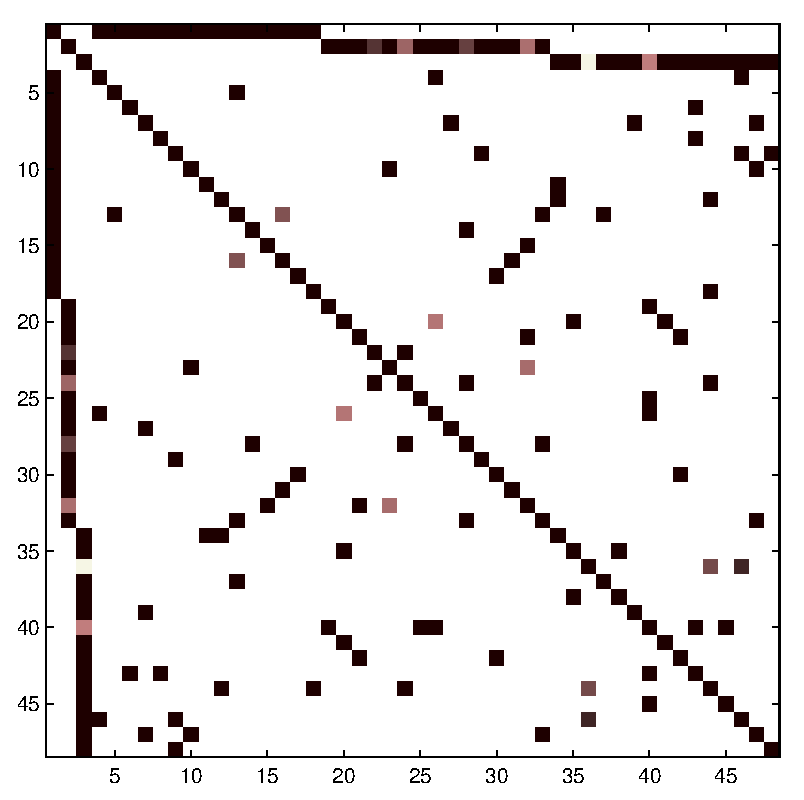
\includegraphics[width=3cm]{fig/disjoint_om}
%  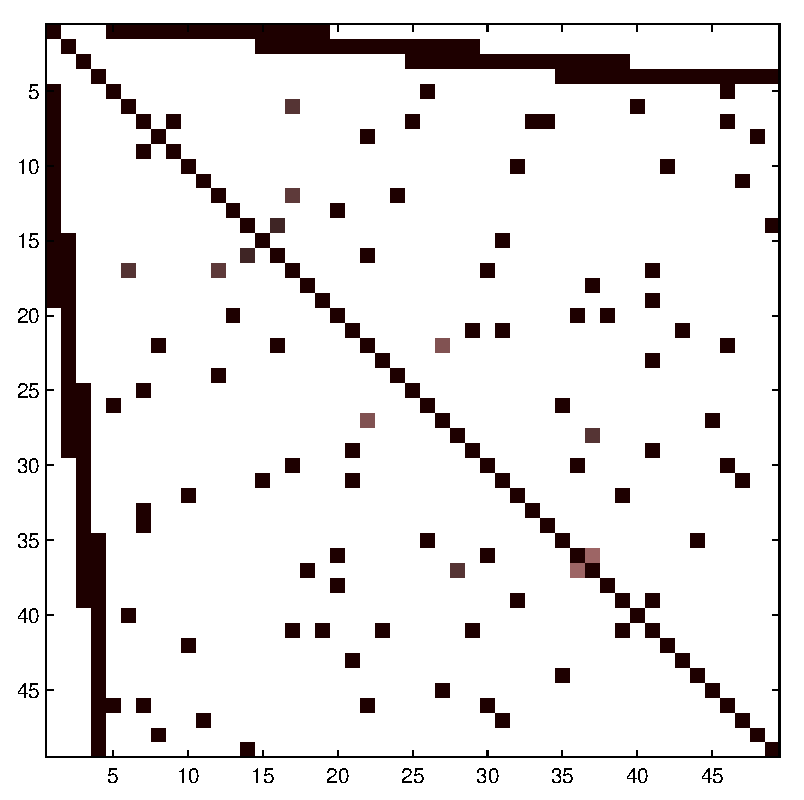
\includegraphics[width=3cm]{fig/overlap_om}
%  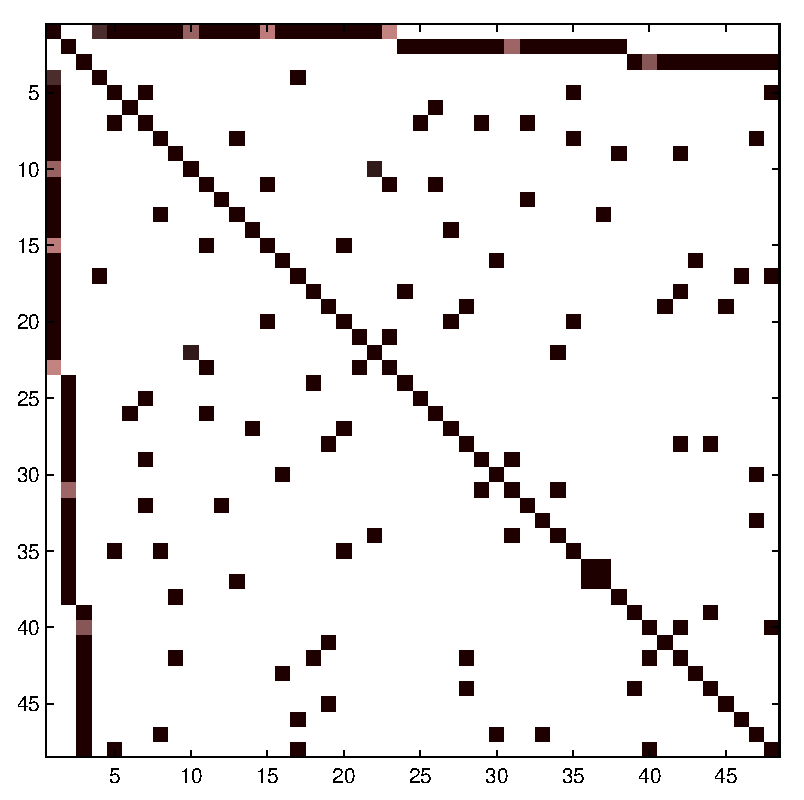
\includegraphics[width=3cm]{fig/diff_om}
%  \end{minipage}
%  \begin{minipage}[ccc]{\linewidth}
%  \includegraphics[width=3cm]{fig/disjoint_tr}
%  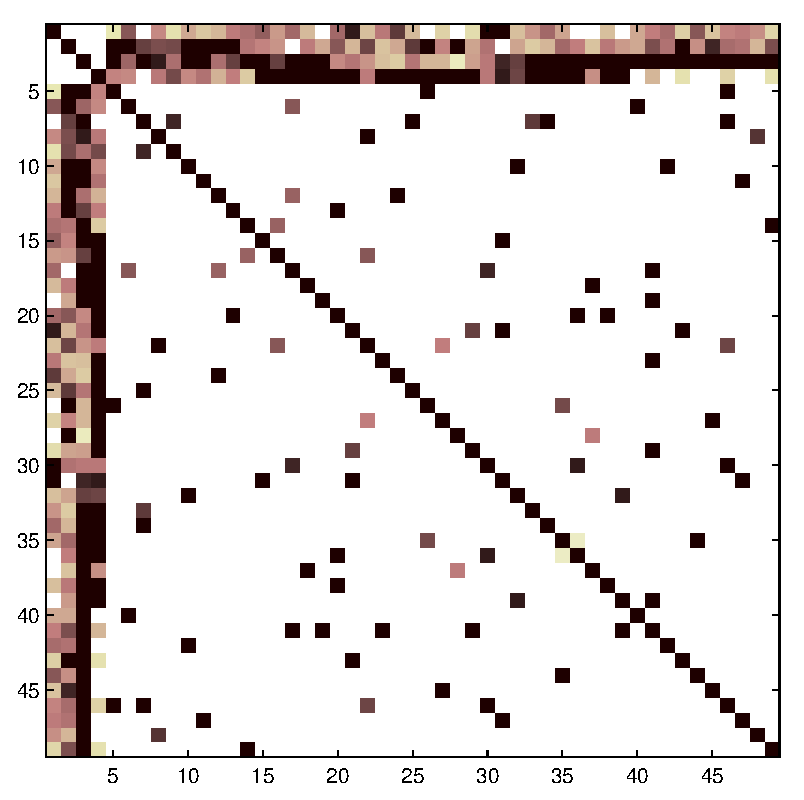
\includegraphics[width=3cm]{fig/overlap_tr}
%  \includegraphics[width=3cm]{fig/diff_tr}
%  \end{minipage}
%  \caption{Experiment for the $k$-chain group Lasso. Top:number of pivots, i.e., drop/full step in active set. Left figure shows the number of pivots per active set call and right plot shows the total number of pivots during iterations. Bottom: evolution of the number of active atoms in our algorithm.}
%\end{figure}

%\begin{figure}
%\center
%\hfill
%\subfigure[Title A]{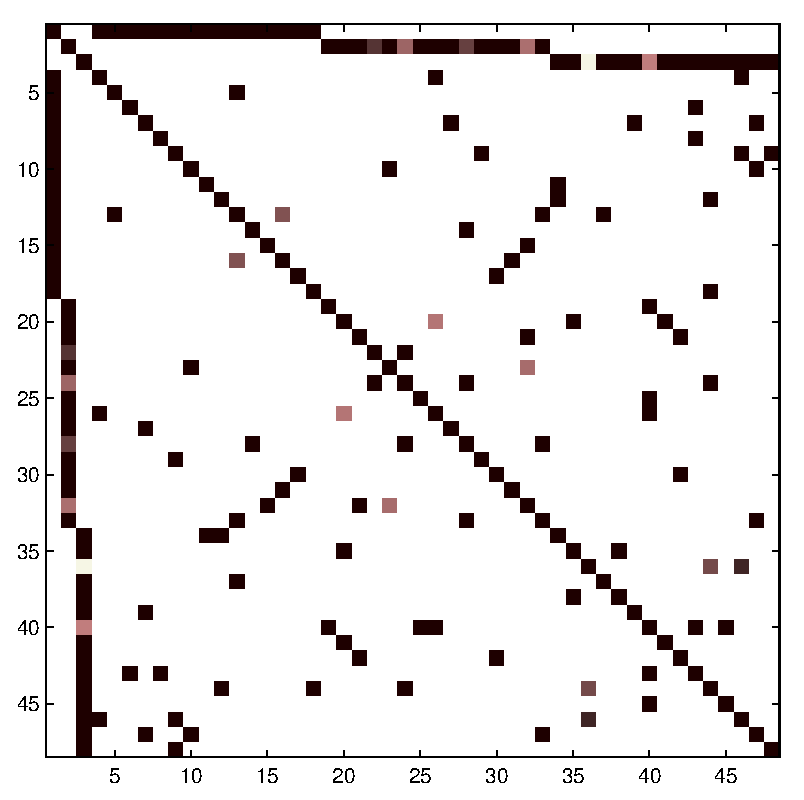
\includegraphics[width=3cm]{fig/disjoint_om}}
%\hfill
%\subfigure[Title B]{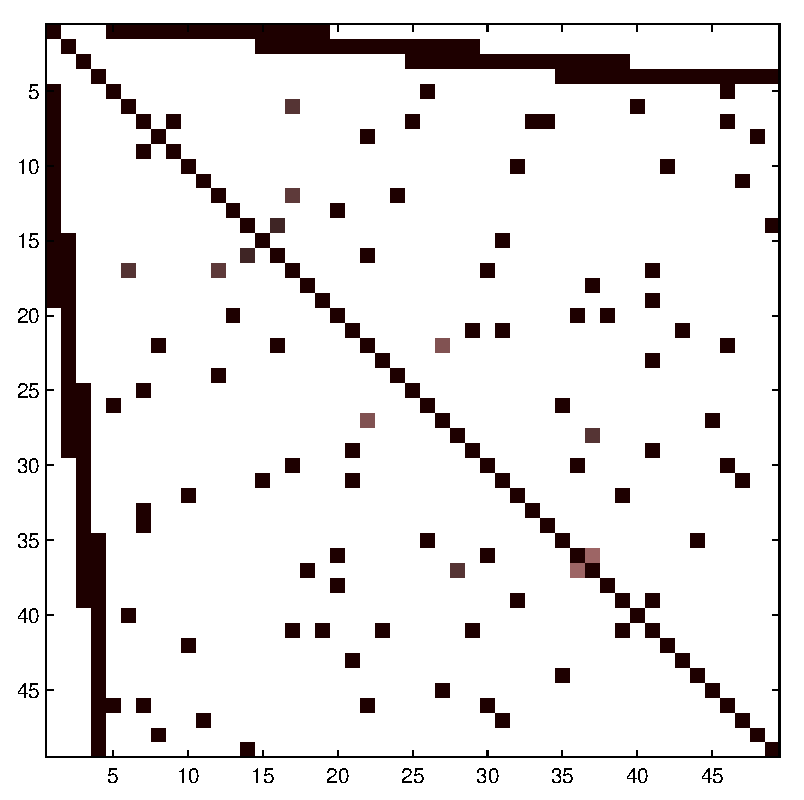
\includegraphics[width=3cm]{fig/overlap_om}}
%\hfill
%\subfigure[Title C]{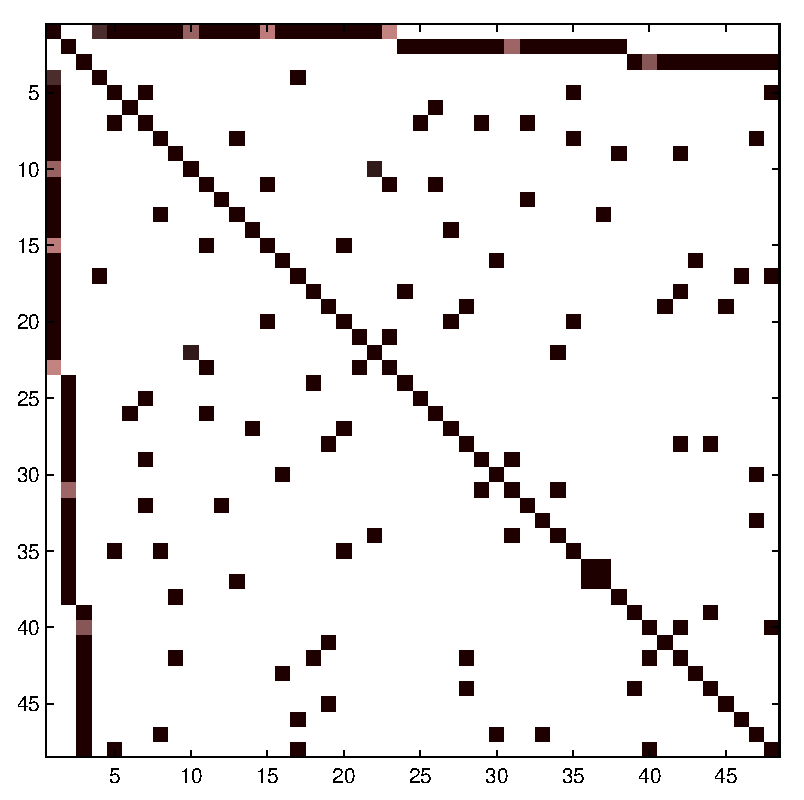
\includegraphics[width=3cm]{fig/diff_om}}
%\hfill
%\\
%\subfigure[Title A]{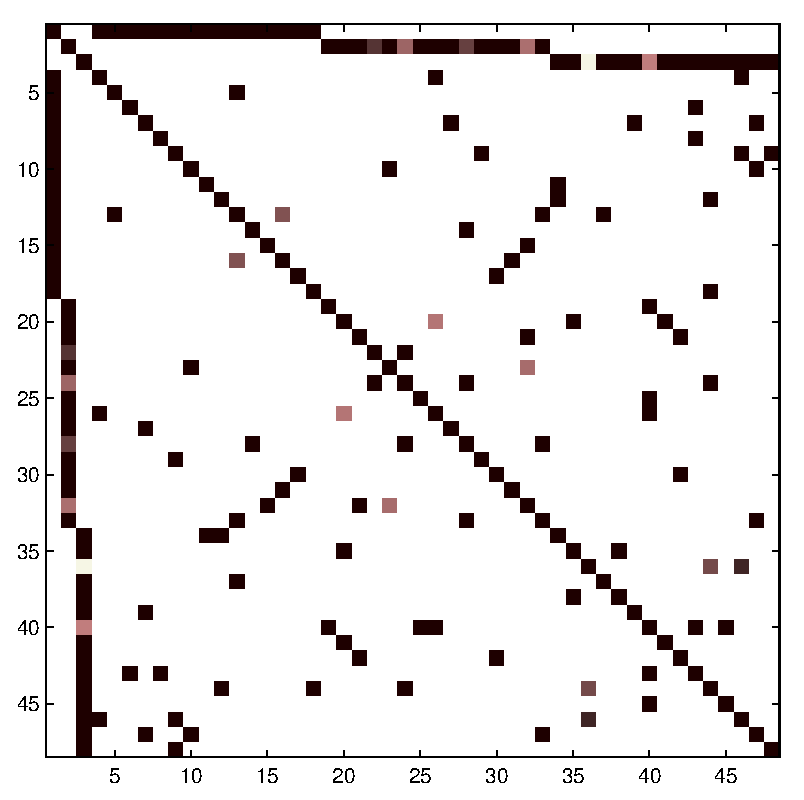
\includegraphics[width=3cm]{fig/disjoint_om}}
%\hfill
%\subfigure[Title B]{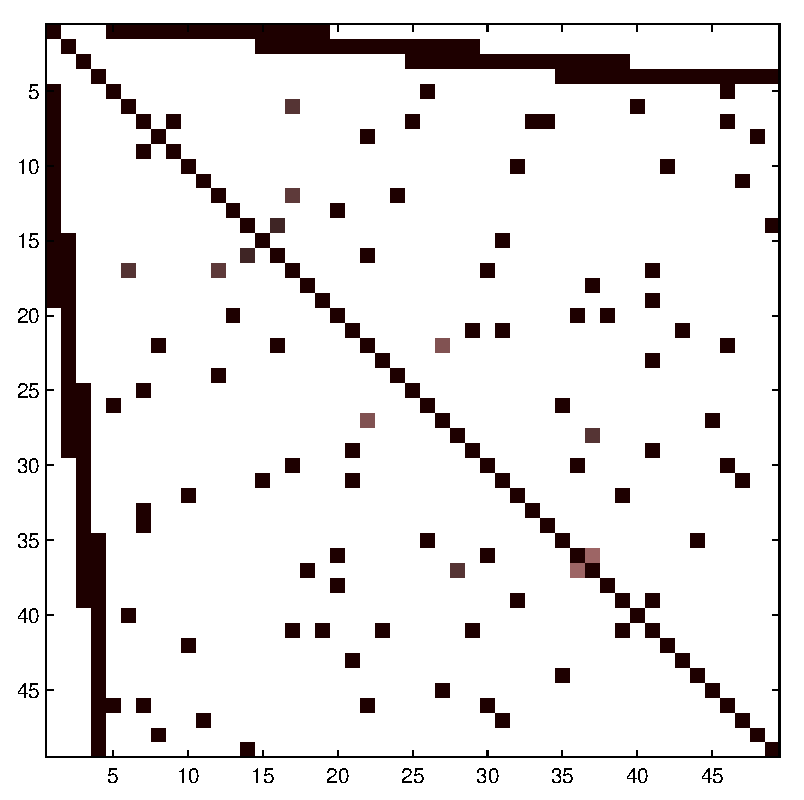
\includegraphics[width=3cm]{fig/overlap_om}}
%\hfill
%\subfigure[Title C]{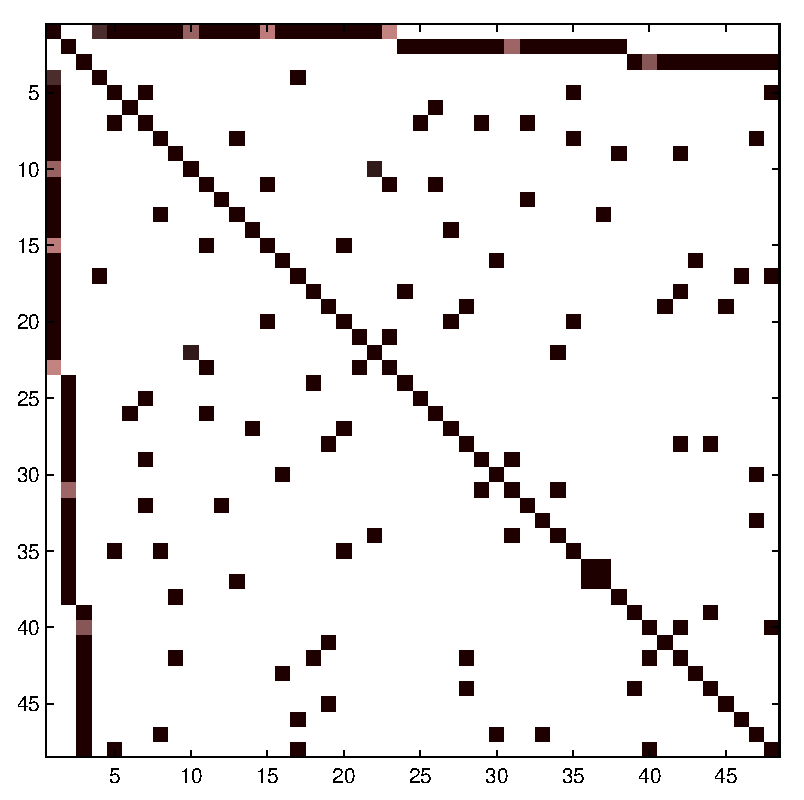
\includegraphics[width=3cm]{fig/diff_om}}
%\hfill
%\caption{Title for both}
%\end{figure}

%\begin{figure}
%\center
%\hfill
%\subfigure[Title A]{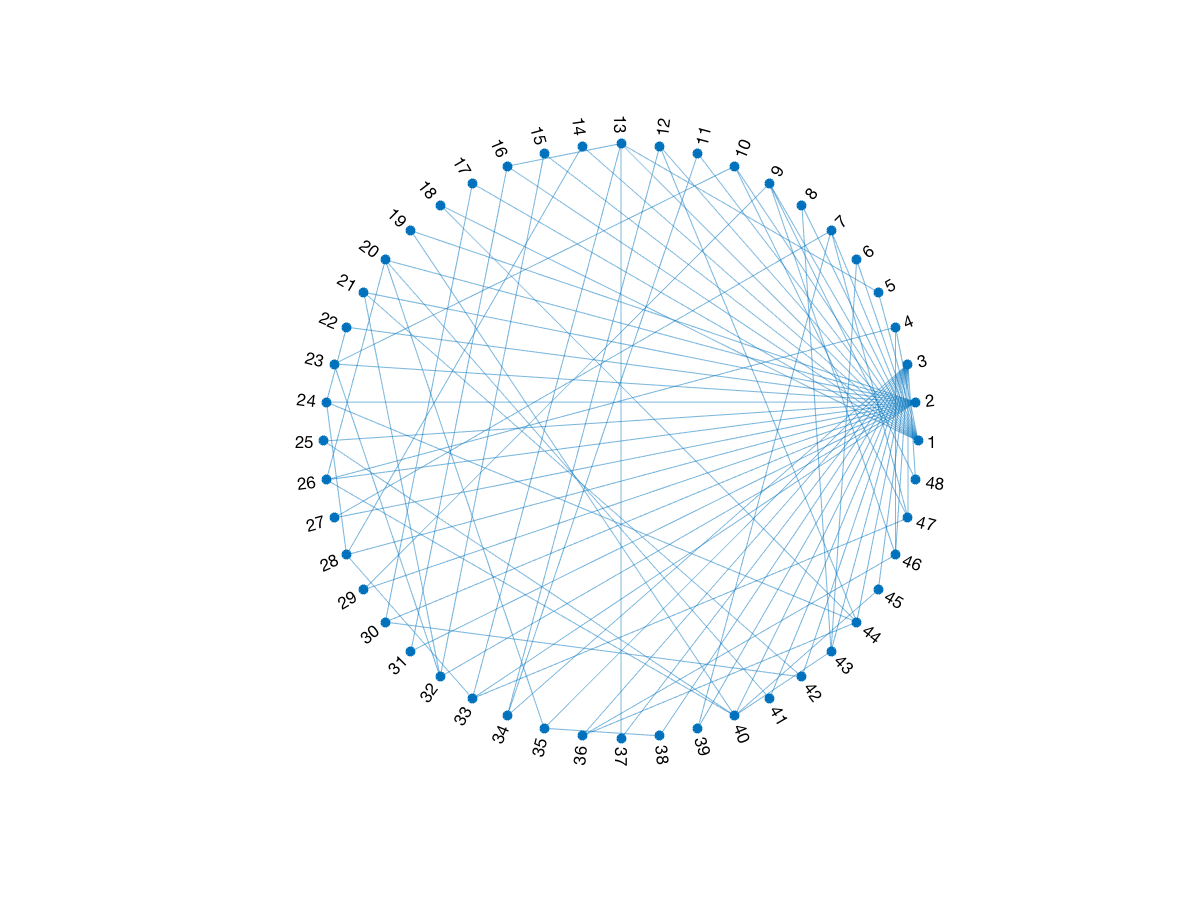
\includegraphics[width=4cm]{fig/disjoint_graph}}
%\hfill
%\subfigure[Title B]{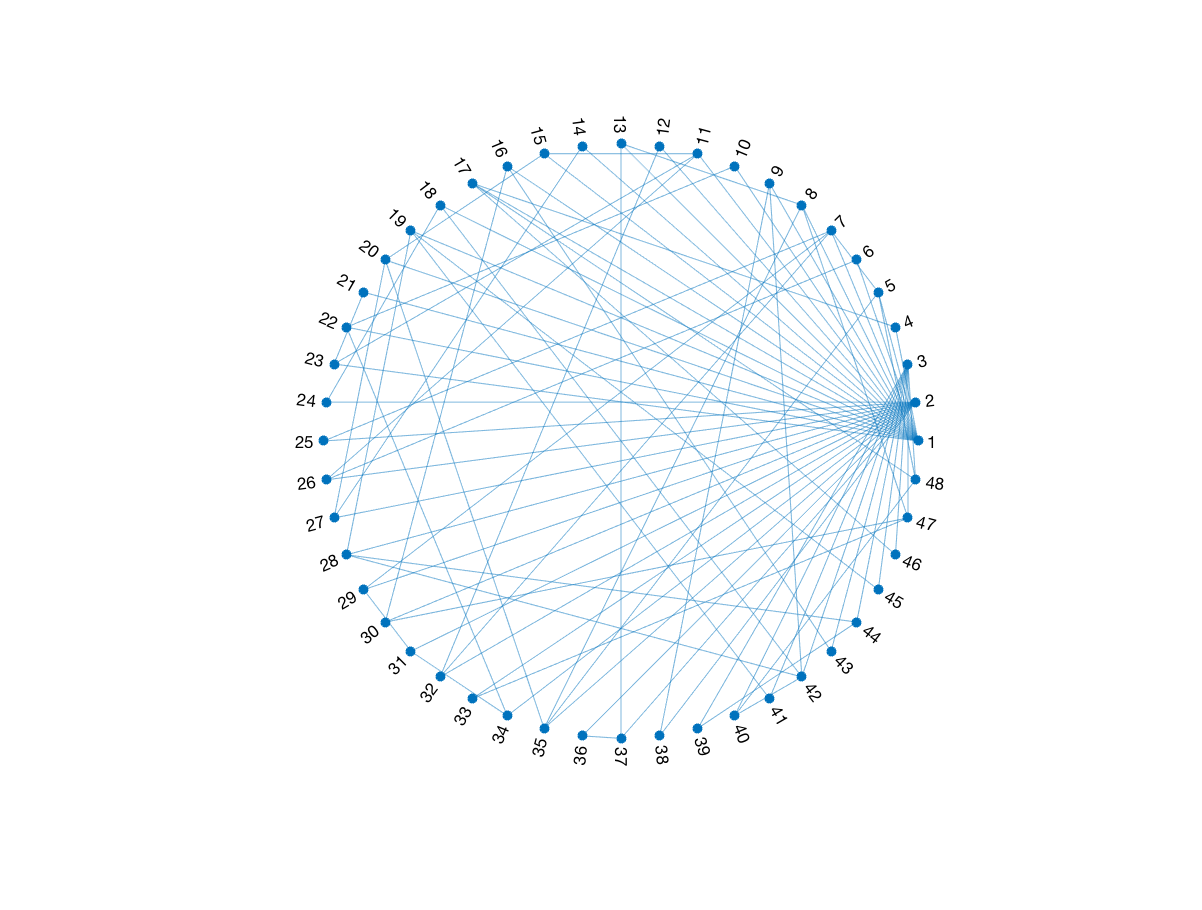
\includegraphics[width=4cm]{fig/diff_graph}}
%\hfill
%\subfigure[Title C]{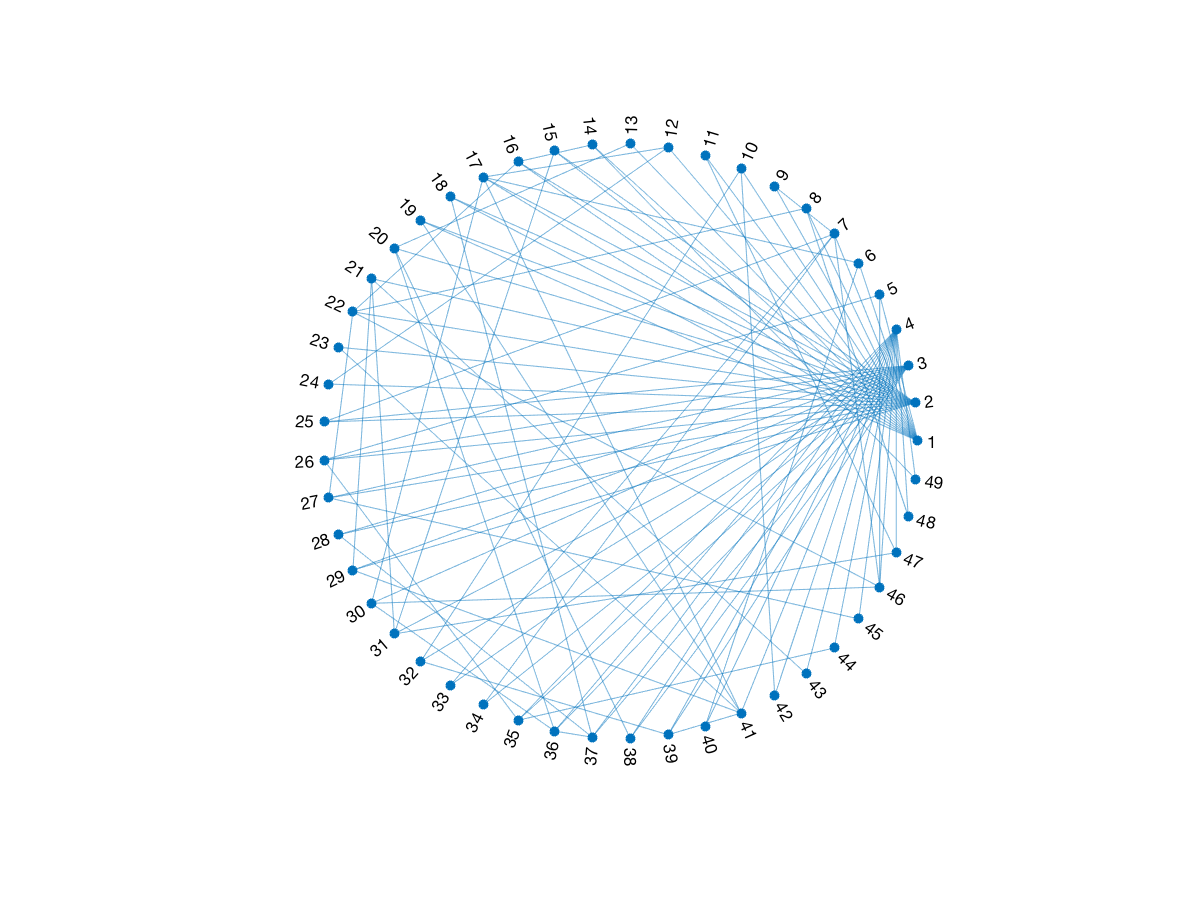
\includegraphics[width=4cm]{fig/over_graph}}
%\caption{Title for both}
%\end{figure}

%\begin{figure}
%\label{fig:synth}
%\center
%\hfill
%\subfigure[ours]{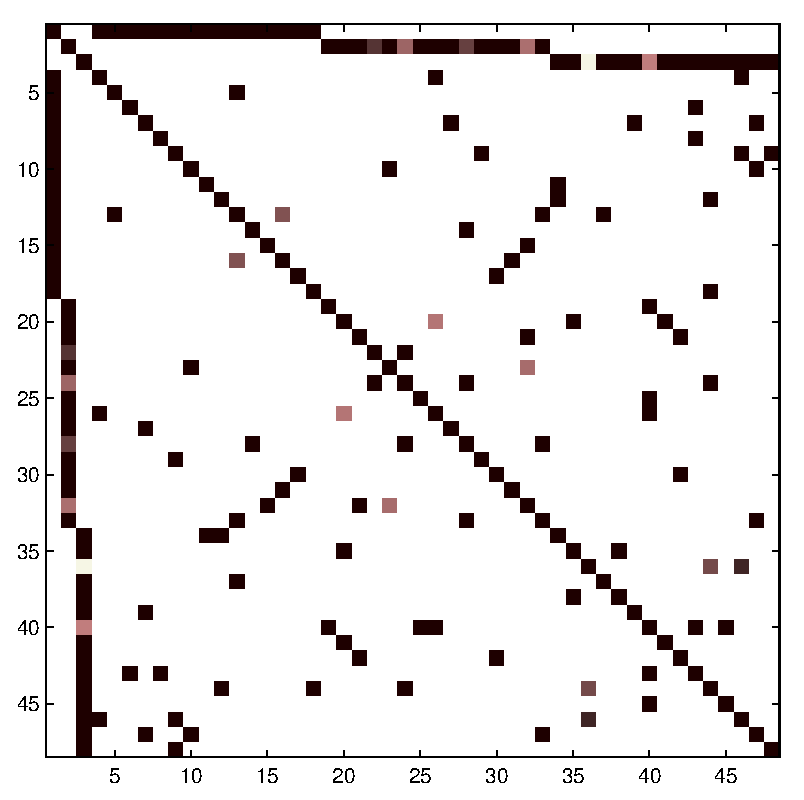
\includegraphics[width=2.2cm]{fig/disjoint_om}}
%\hfill
%\subfigure[$\ell_1+\tr$]{\includegraphics[width=2.2cm]{fig/disjoint_tr}}
%\hfill
%\subfigure[ours]{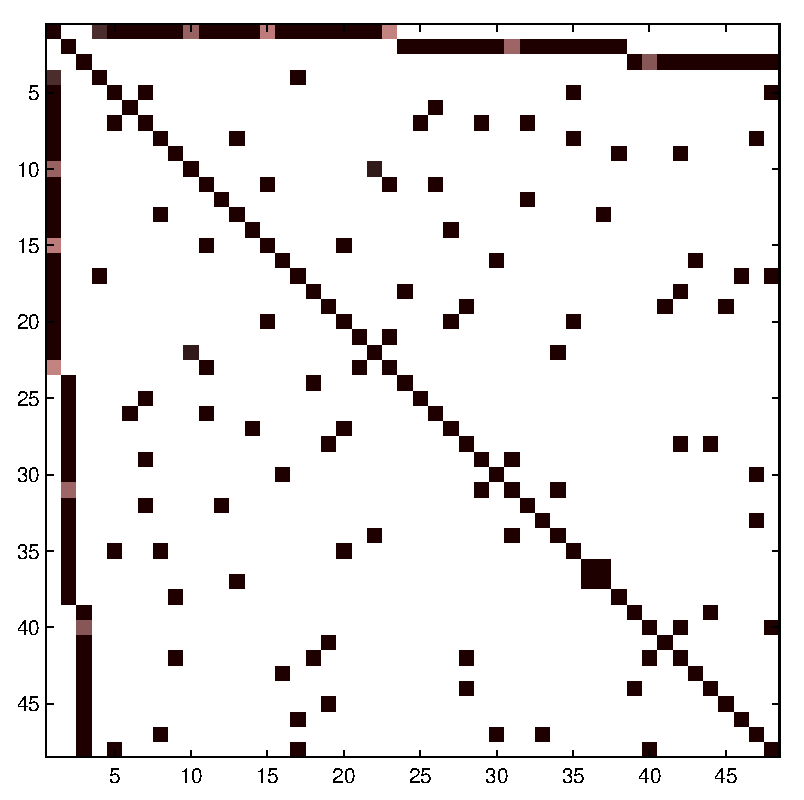
\includegraphics[width=2.2cm]{fig/diff_om}}
%\hfill
%\\
%\subfigure[$\ell_1+\tr$]{\includegraphics[width=2.2cm]{fig/diff_tr}}
%\hfill
%\subfigure[ours]{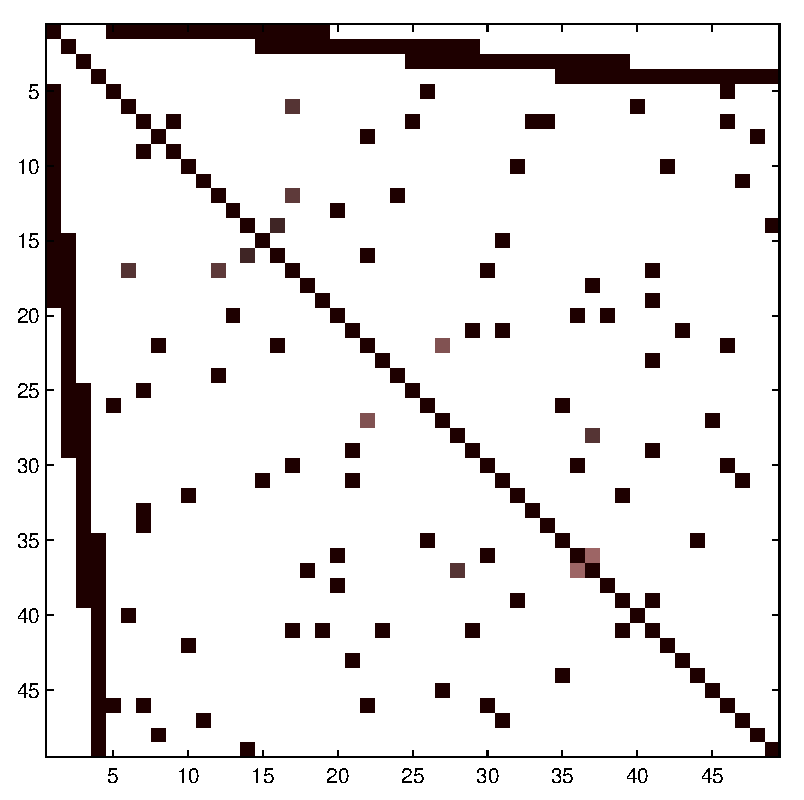
\includegraphics[width=2.2cm]{fig/overlap_om}}
%\hfill
%\subfigure[$\ell_1+\tr$]{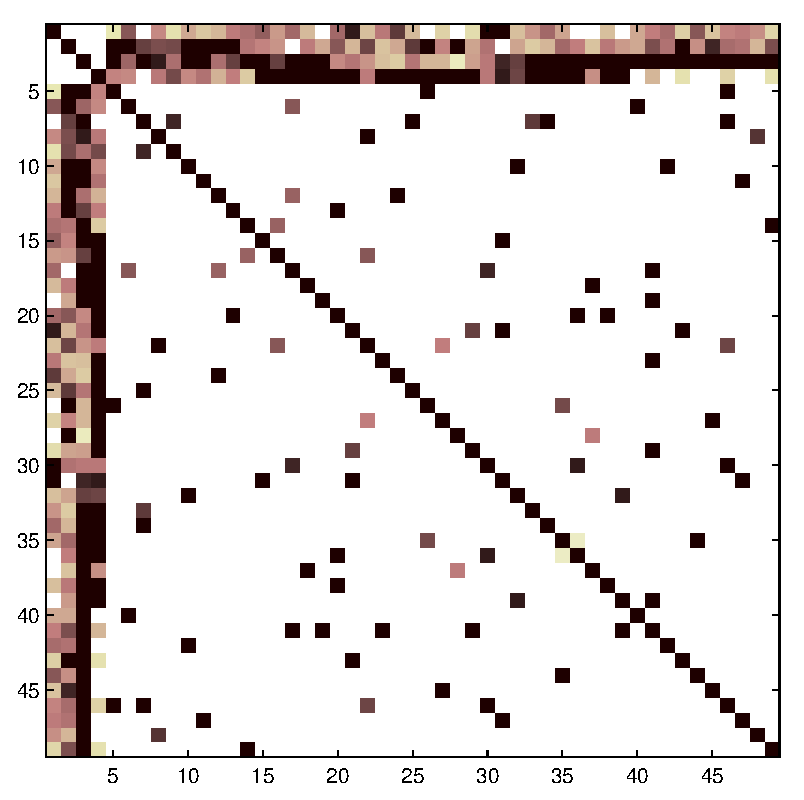
\includegraphics[width=2.2cm]{fig/overlap_tr}}
%\hfill
%\caption{Estimated complete concentration matrices: for \textit{model 1} in (a) ours and (b) $\ell_1+\tr$ regularization; for \textit{model 2} in (c) ours and (d) $\ell_1+\tr$ regularization; for \textit{model 3} in (e) ours and (f) $\ell_1+\tr$ regularization }
%\end{figure}



\begin{figure}
\label{fig:synth}
\center
\begin{tabular}{ccc}
  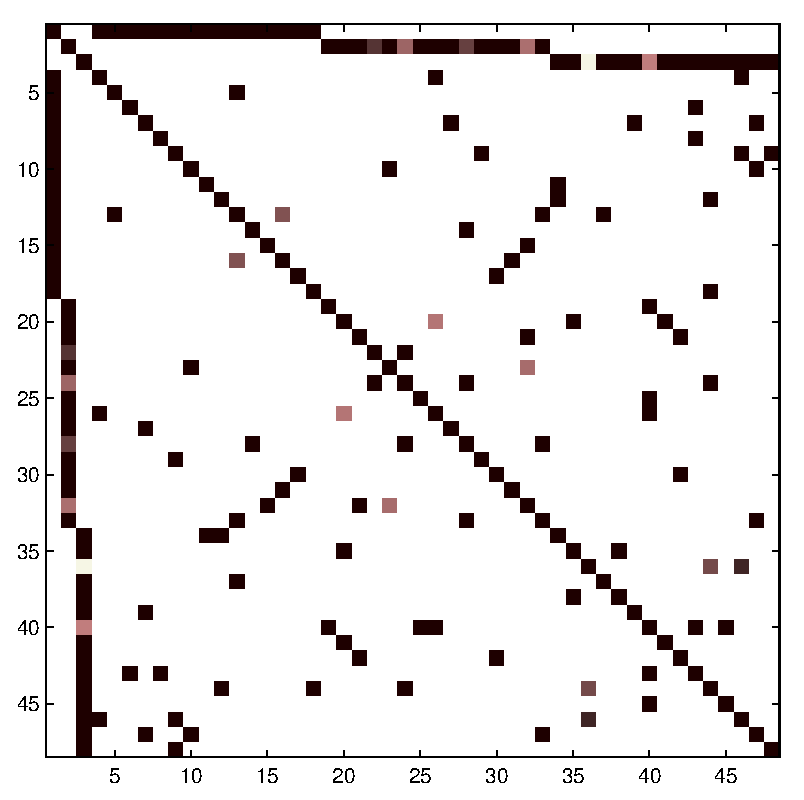
\includegraphics[width=3.5cm]{fig/disjoint_om} 
  &   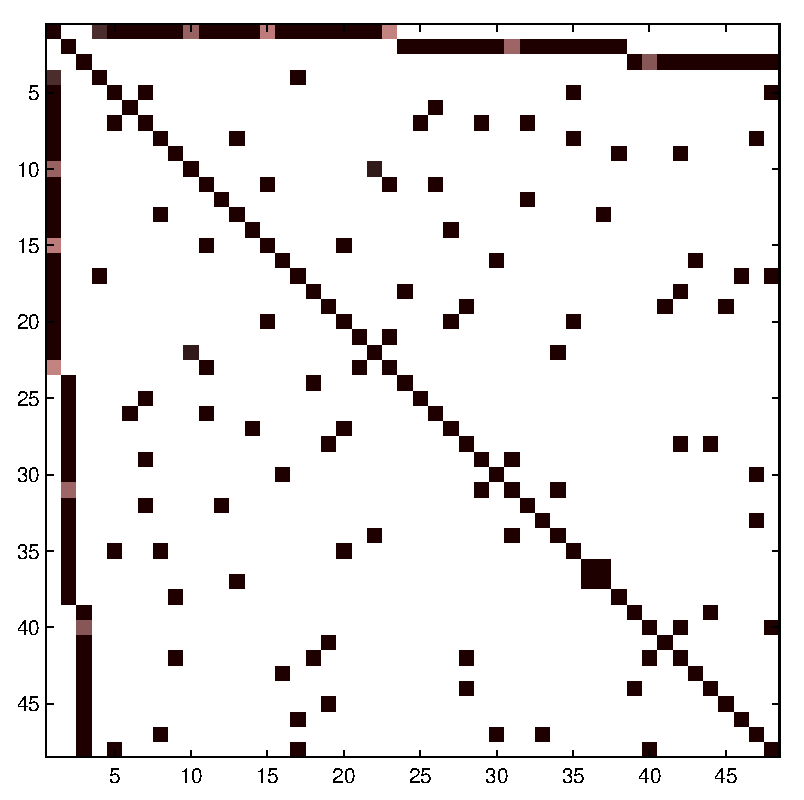
\includegraphics[width=3.5cm]{fig/diff_om}
  &   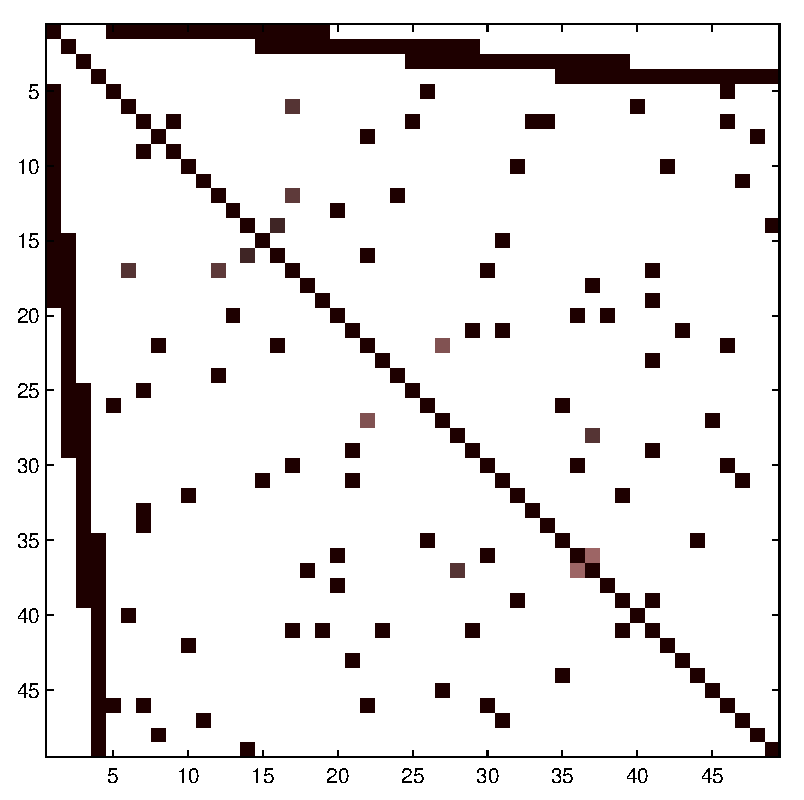
\includegraphics[width=3.5cm]{fig/overlap_om}
   \\    (a) \textit{model 1}, ours & (b)  \textit{model 2}, ours  & (c)  \textit{model 3}, ours  \\[6pt]
 \includegraphics[width=3.5cm]{fig/disjoint_tr} 
  &   \includegraphics[width=3.5cm]{fig/diff_tr}
  &   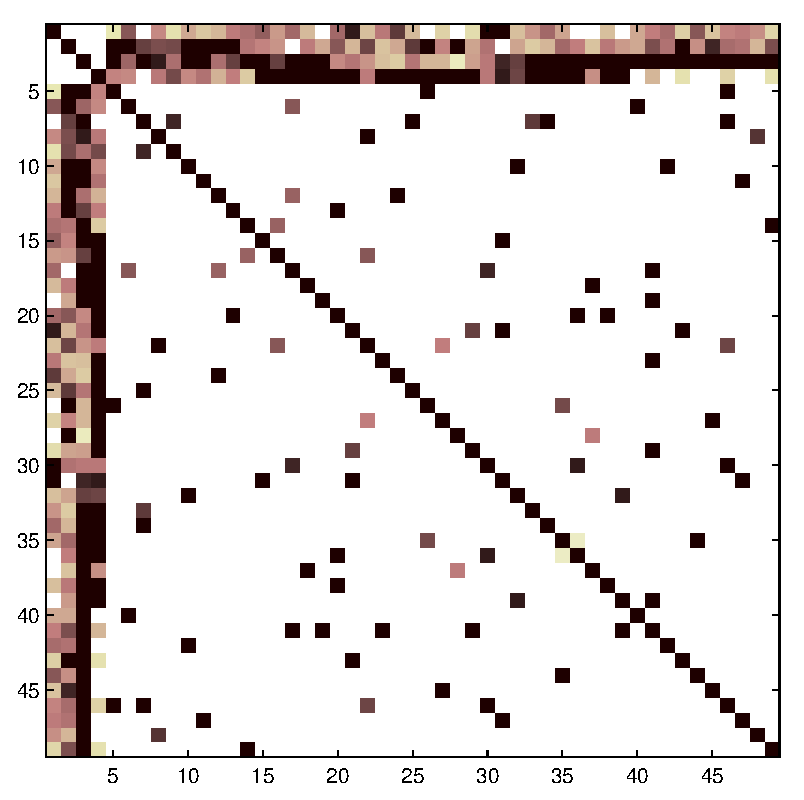
\includegraphics[width=3.5cm]{fig/overlap_tr}
   \\    (d)  \textit{model 1}, $\ell_1+\tr$ & (e)  \textit{model 2}, $\ell_1+\tr$  & (f)  \textit{model 3}, $\ell_1+\tr$  \\[6pt]
\end{tabular}
\caption{Estimated complete concentration matrices: for \textit{model 1} in (a) ours and (d) $\ell_1+\tr$ regularization; for \textit{model 2} in (b) ours and (e) $\ell_1+\tr$ regularization; for \textit{model 3} in (c) ours and (f) $\ell_1+\tr$ regularization }
\end{figure}


\subsection{Microarray dataset}

We consider the MILE data \citep{haferlach2010clinical} that measure the mRNA expression levels of 16,853 genes in 541 patients with acute myeloid leukemia (AML), an aggressive blood cancer. We selected 250 genes in total, the ones with higher variance and  also genes highly associated with AML: FLT3, NPM1, CEBPA, KIT, N-RAS, MLL, WT1. We fix the size of the blocks to $k=100$ for our method. Figure \ref{fig:gen} shows qualitative results. 

\begin{figure}
\label{fig:gen}
\center
\begin{tabular}{cccc}
      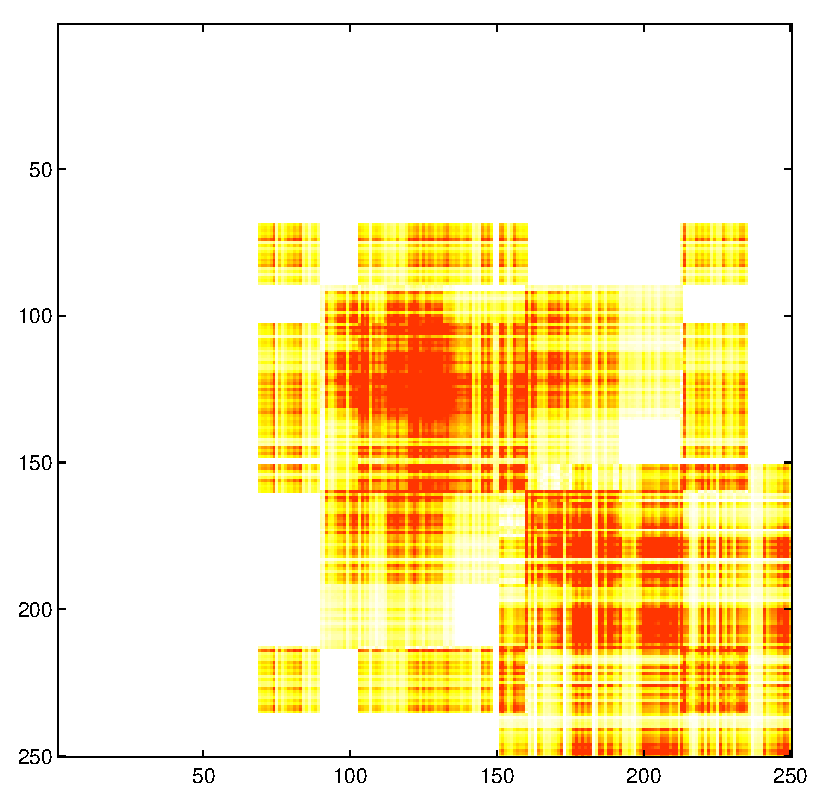
\includegraphics[width=4cm]{fig/MILE_Lom}
  &   \includegraphics[height=3.8cm]{fig/MILE_blocks}
  &   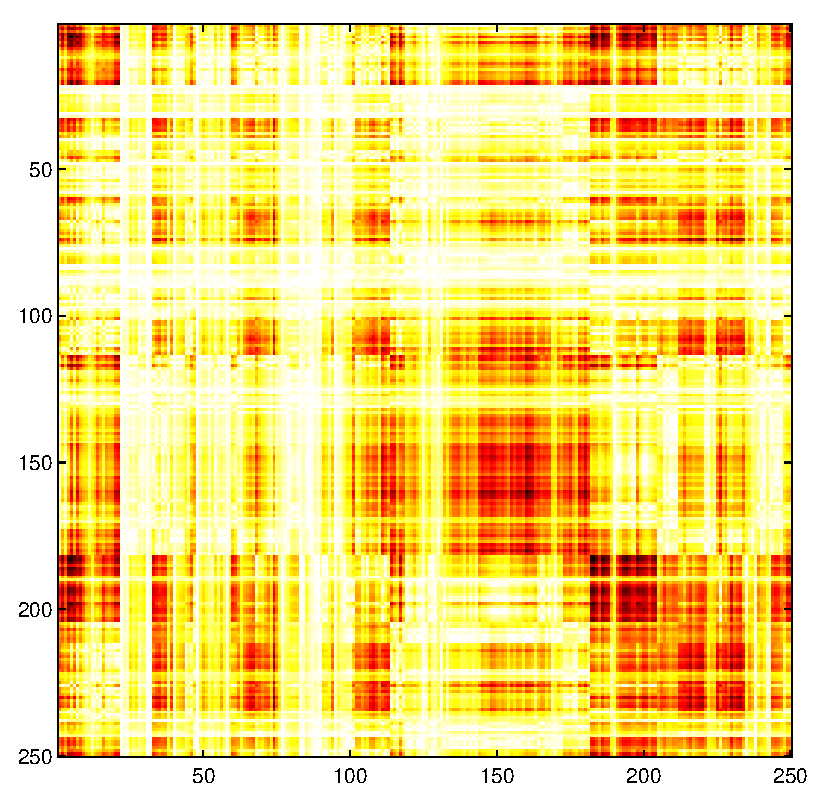
\includegraphics[width=4cm]{fig/MILE_Lsl_not_ordered} 
  &   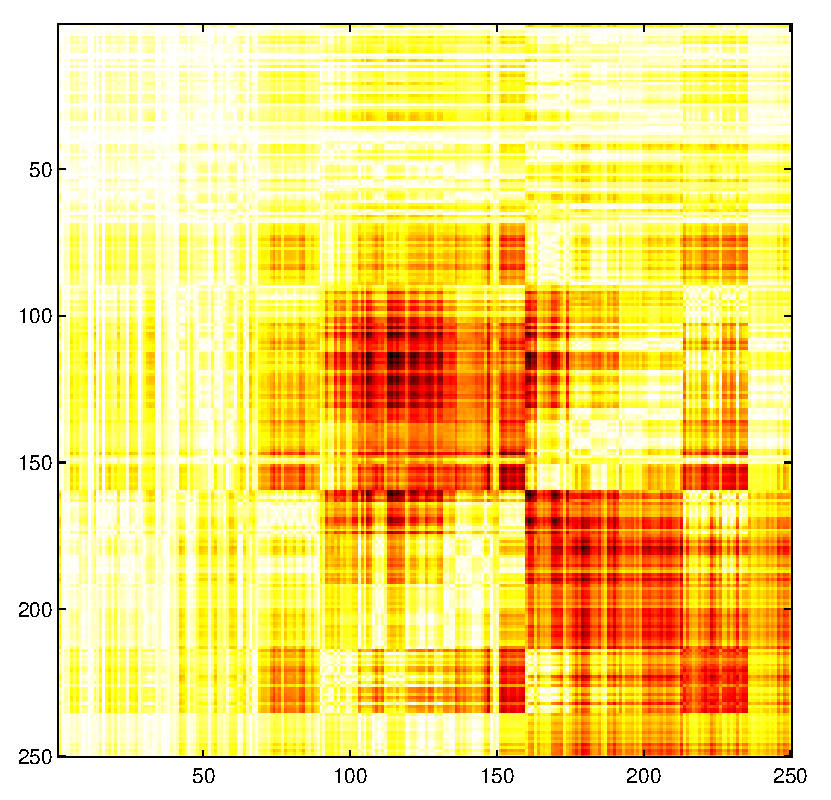
\includegraphics[width=4cm]{fig/MILE_Lsl_ordered} 
   \\   (a)  $\hat{L}$ ours  & (b) blocks &(c) $\hat{L}$ for $\ell_1+\tr$ &(d) $\hat{L}$ for $\ell_1+\tr$ ordered  
\end{tabular}
\caption{Estimated low rank component for our method (a) and the support of the 4 rank-one 100-sparse components $uu^{\top}$  (b).  Estimated low rank component for maximum log-likelihood regularized by $\ell_1+\tr$ (d) and the same estimated where reordered (same order as the one in (a), revealed by the block structure) }
\end{figure}
